\documentclass[../../main]{subfiles}
\begin{document}
The manufacturing industry is undergoing a digital transformation, driven by advancements in technologies like artificial intelligence, autonomous robots, and the Internet of Things. These innovations aim to enhance efficiency, productivity, and competitiveness in industrial processes. TEKNOFEST’s Digital Technologies in Industry Competition challenges participants to design an autonomous guided robot for factory logistics, addressing real-world tasks such as navigation, load handling, and mapping. This report explores the strategies used to overcome these challenges and achieve the competition’s objectives. By doing so, it highlights the critical role of digitalization in advancing industrial automation and fostering innovation.

\section{TEKNOFEST competition Rules}
The following rule apply to the operation of guided robots during the competition:

\subsection{ Autonomous Operation}
The guided robot must perform all tasks autonomously within the specified scenarios, including line-following.

\subsection{Overload Warning}
The robot must issue an overload warning if it lifts a load exceeding the specified limit and continue carrying the load only after the weight is reduced below the limit.
\newpage
\subsection{Charging Task}
If the robot's charge level falls below a certain threshold, teams can earn additional points by having the robot autonomously navigate to the charging area and begin charging. Teams must inform the jury in advance if they wish to perform this task, which will be conducted at a time deemed appropriate by the jury.

\subsection{Obstacle Navigation}
The robot should autonomously stop at loading/unloading points and navigate around obstacles if they are not removed. Obstacles will be detected by sensors, and the robot must stop at an appropriate distance. If the obstacle remains, the robot should autonomously go around it and complete its tasks.

\subsection{QRCODE Labels}
QRCODE labels at loading and unloading positions must be readable by appropriate sensors on the robot.

\subsection{Control Screen (GUI)}
Teams must prepare a graphical user interface (GUI) that allows them to monitor the vehicle’s status and issue commands when necessary. However, interventions via the control panel will incur penalty points.

\subsection{No Manual Control}
The robot cannot be controlled by joysticks, portable hand controls, phones, or tablets.

\subsection{Load Handling Display}
The pick-up or dropping of loads must be displayed on the control panel (GUI) using sensors.


\subsection{Mapping for Advanced Competitors}
Advanced-level competitors are required to map the track. For mapping, advanced teams will be given a specific amount of time after the loaded course is revealed. The teams are expected to map and display the competition area within the allocated time. 

Mapping should be performed using devices such as laptops and tablets belonging to the team members at the control desk. Additionally, teams are expected to create a control panel (GUI) that displays competition details such as speed and total task time. The mapping should be detailed, and QRCODE labels should be displayed on the map as they are read.
\begin{figure}[h!]
    \centering
    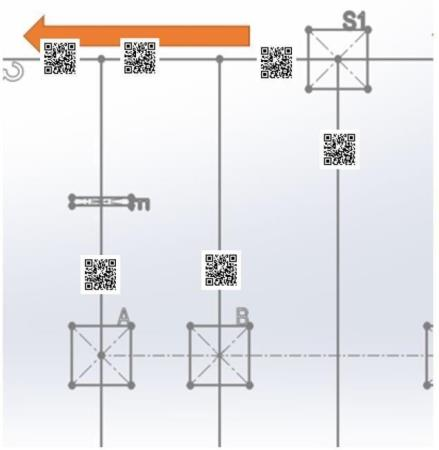
\includegraphics[width=0.4\textwidth]{img/qr.jpg}
    \caption{QRCODE Layout}
    \label{fig:tekno}
\end{figure}
\section{DETAILS OF THE COMPETITION AREA}

For the competition, there will be 2 rectangular-shaped representative factory areas of approximately 150 square metres each. These areas will include a track representing the layout of roads and internal logistics roads. Additionally, there will be a separate area where a table is located for each participating competitor team to use. The following details apply:

\subsection{Power Supply}
The competition area will have a 220 VAC power supply. A control desk will be located at the edge of the track for the competing team to control their guided robot. At the control desk, 220 VAC voltage will be provided, and each team is responsible for performing AC/DC conversion using their own converter. The highest DC voltage level that can be used is 50V.


\subsection{Track Layout}
The track will resemble a factory area with designated pick-up and drop-off points. The distribution of these points may vary for each competing team, as determined by the referees. The track area will consist of two similar sections, allowing two different teams to compete simultaneously.

\newpage
\subsection{Sample View of the Track}
The sample view of the track will be provided separately for reference(\cref{fig:tekno2}).

\begin{figure}[h!]
    \centering
    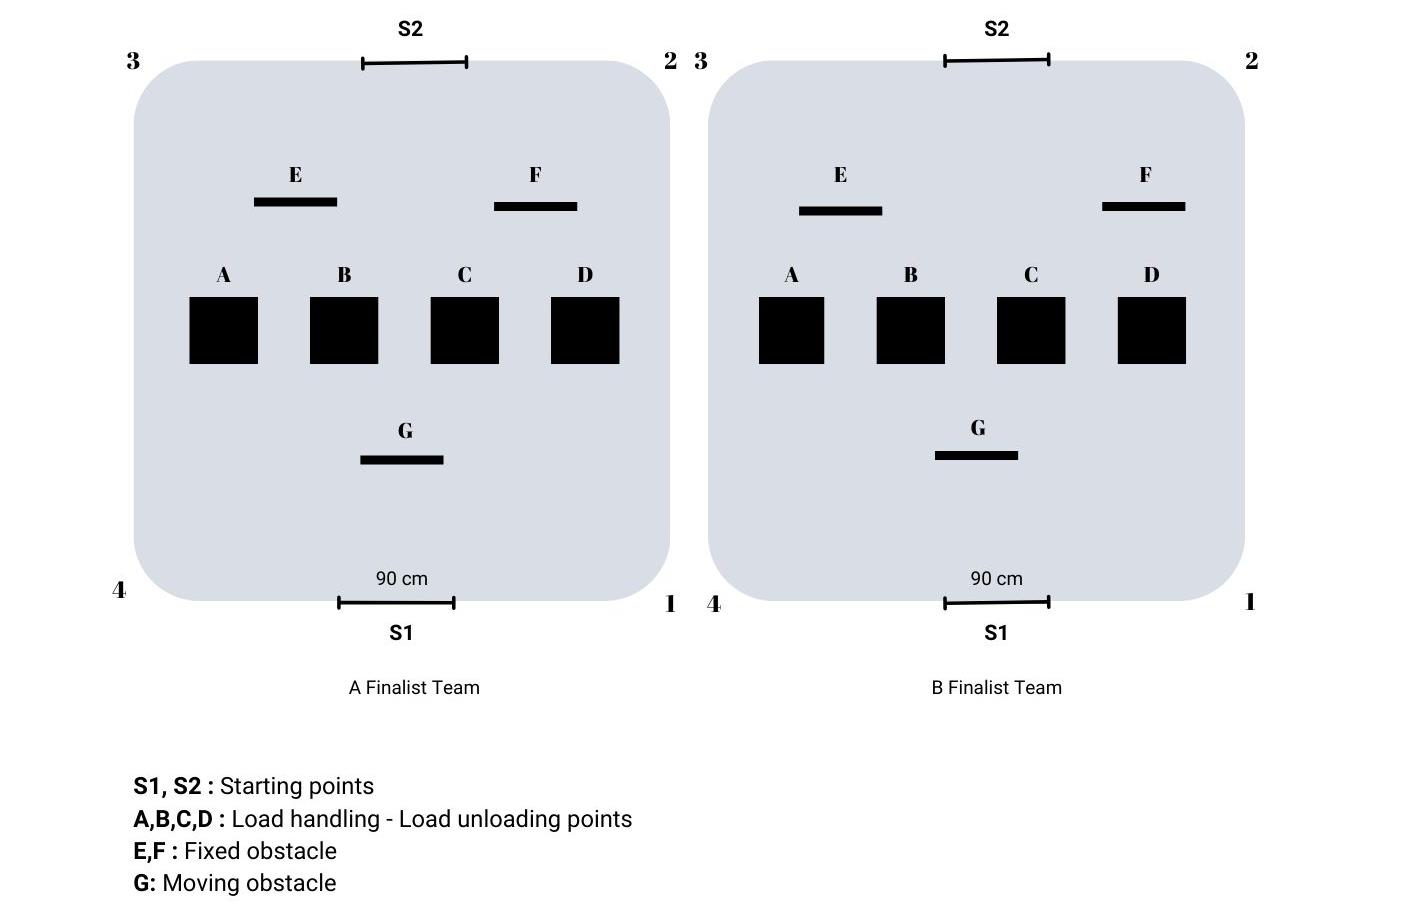
\includegraphics[width=\textwidth]{img/cmparea.jpg}
    \caption{Sample Track Area}
    \label{fig:tekno2}
\end{figure}
\section[Load Handling Robot Specs \& Limits]{LOAD HANDLING ROBOT TECHNICAL SPECIFICATIONS AND LIMITATIONS}

The maximum dimensions of the load handling robot are as follows: 1,000 mm in length, 900 mm in width, and 500 mm in height. The dimensions of the load handling robots must not exceed these specified limits. However, when the mechanism used to lift the load platform is operated, the robot may exceed the height limit. The height restriction applies only to the situation where the vehicle is not operating under load.

The maximum load amount that robots must carry is 125 kg. Robots that lift more than 125 kg and do not provide an overload warning will be deemed to have failed to fulfill this task. The competition organization will provide loads with dimensions of 30 cm x 30 cm x 10 cm (\cref{fig:tekno}a)and a weight of 25 kg each. These loads will be placed on a platform with a maximum height of 50 cm from the ground)(\cref{fig:tekno3}b), allowing the robot to easily position itself underneath and lift the load from all directions. The weight of the load platform provided by the competition organization will also be 25 kg.

The positions for load pick-up and drop-off will be defined using QRCODE tags. These tags will ensure precise identification of the designated locations for the robot to perform its tasks.
\begin{figure}[h!]
    \centering
    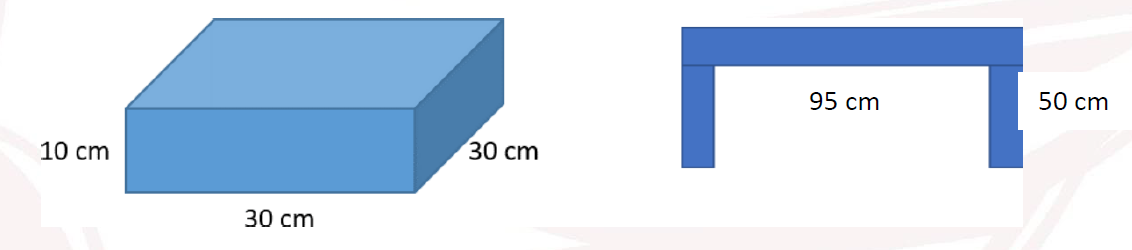
\includegraphics[width=\textwidth]{img/load.png}
    \caption{Load (a) and platform (b)}
    \label{fig:tekno3}
\end{figure}

\section{Sample Scenario}

The robot must first navigate around the corner points according to the scenario type, starting from the initial position without any load, and return to the starting point. During this process, teams are required to complete the mapping task. A total of four unloaded scenarios are illustrated in \cref{sample loaded scenario}.

Following the unloaded navigation, the robot should proceed to point A from the starting point to pick up a load and then continue to point C. Upon reaching point C, the robot must leave the load there and proceed to point D without carrying any load. After arriving at point D, the robot should pick up another load and transport it to point B. Once the load is delivered at point B, the robot must complete the task by returning to the starting point without any load. \cref{Example No Load Scenario} depicts four loaded scenarios, which vary depending on the starting points.
\begin{figure}
    \centering
    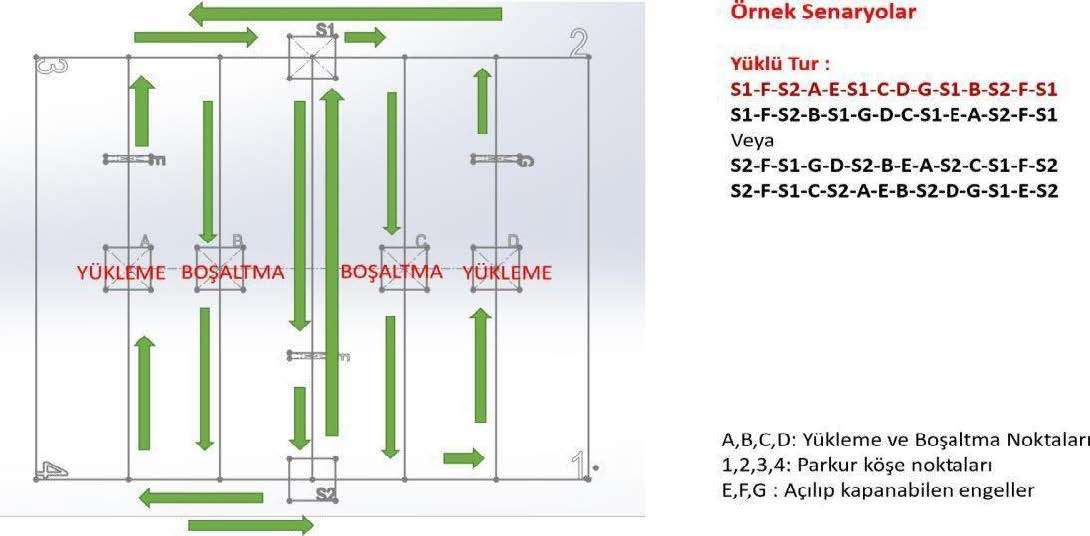
\includegraphics[width=\textwidth]{img/samplTK.jpg}
    \caption{Sample Loaded Scenario}
    \label{sample loaded scenario}
\end{figure}
\begin{figure}[h!]
    \centering
    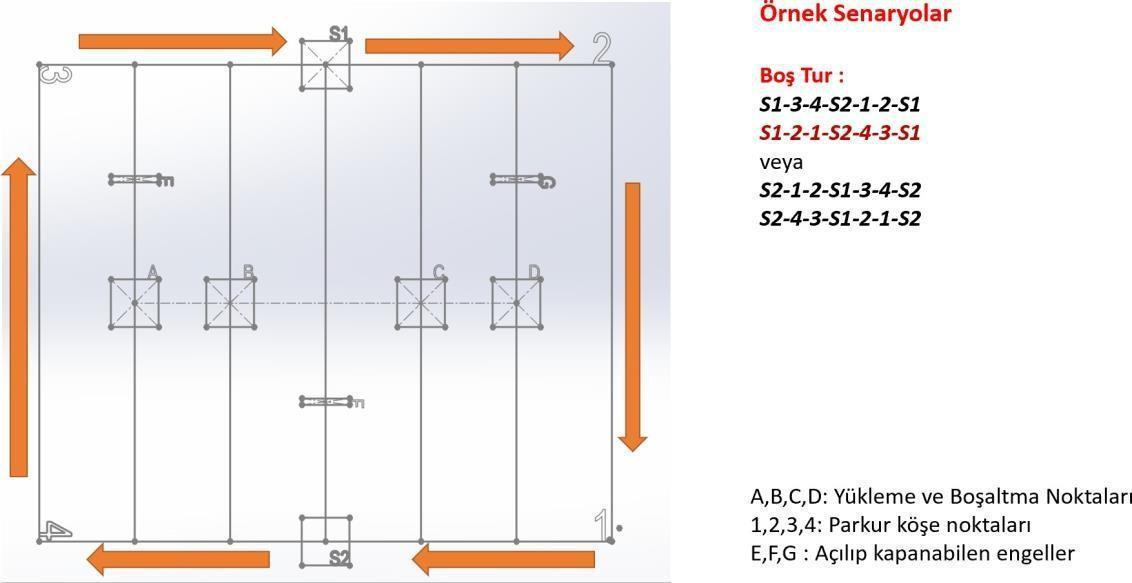
\includegraphics[width=1\textwidth]{img/mmapingTk.jpg}
    \caption{Example No Load Scenario}
    \label{Example No Load Scenario}
\end{figure}
\end{document}